\documentclass{book}

\usepackage[shortsuper,hacm,ltfont]{common/uruwi}

\newcommand{\lname}{aaaaaaaaaaA}

\title{lek-\bs{}tsaro-ma sil lek-ma sil se\^otxe-\bs{}ri\^umako}
\author{uruwi}

\begin{document}

\pagecolor{Thistle!25}

\begin{titlepage}
    \makeatletter
    \begin{center}
        {\color{Orchid} \hprule \vspace{1.5ex} \\}
        {\Huge \ltfont \textcolor{Plum}{LKe\bs{}TSxaRMoa SL LKeMa SL STfXe\bs{}RMyaKo}\\}
        {\large \kardinal \textcolor{Purple}{\@title} \\}
        {\large \textit{\lname}, the language of \textit{Rymako} \\}
        {\color{Orchid} \hprule \vspace{1.5ex} \\}
        % ----------------------------------------------------------------
        \vspace{1.5cm}
        {\Large\bfseries \@author}\\[5pt]
        %uruwi@protonmail.com\\[14pt]
        % ----------------------------------------------------------------
        \vspace{2cm}
        \textkardinal{aaaaaaaaaaaaaaaaa} \\
        {aaaaaaaaaaaaaaaaa} \\[5pt]
        \emph{A complete grammar}\\[2cm]
        %{in partial fulfilment for the award of the degree of} \\[2cm]
        %\tsc{\Large{{Doctor of Philosophy}}} \\[5pt]
        %{in some subject} \vspace{0.4cm} \\[2cm]
        % {By}\\[5pt] {\Large \sc {Me}}
        \vfill
        % ----------------------------------------------------------------
        %\includegraphics[width=0.19\textwidth]{example-image-a}\\[5pt]
        %{blah}\\[5pt]
        %{blahblah}\\[5pt]
        %{blahblah}\\
        \vfill
        {\@date}
    \end{center}
    \makeatother
\end{titlepage}

\pagecolor{Thistle!15}

\begin{center}
    \textit{Dedicated to Isoraķatheð.}
\end{center}

\begin{verbatim}
Branch: canon
Version: 0.1
Date: 2017-09-12
\end{verbatim}

(C)opyright 2017 Uruwi. See README.md for details.

\tableofcontents

\section{Introduction}

\chapter{Phonology and orthography}

\section{Phoneme inventory}

\begin{table}[h]
    \caption{The consonants of \lname.}
    \centering
    \begin{tabular}{|l|l|l|l|l|l|}
        \hline
        & Bilabial & Alveolar & Palatal & Velar & Glottal \\
        \hline
        Nasal & m & n & ɲ & ŋ & \invalid \\
        Plosive & p b & t d & c ɟ & k ɡ & ʔ \\
        Fricative & f & s & ʃ & x & \\
        (coarticulated) & θx & fx & & fʃ & \invalid \\
        Affricate & & ts & tʃ & & \\
        Lateral fricative & \invalid & ɬ & & & \invalid \\
        Approximant & & ɹ & j & w & \\
        Lateral approximant & \invalid & l & & & \invalid \\
        Trill & & r & & \invalid & \invalid \\
        \hline
    \end{tabular}
\end{table}
\begin{table}[h]
\centering
    \caption{The vowels of \lname.}
    \begin{tabular}{|l|l|l|}
        \hline
        Spread & Half-rounded & Rounded \\
        \hline
        i & y̜  & y \\
        ɯ & u̜ & u \\
        ɛ & & œ \\
        ʌ & & ɔ \\
        ä & & \\
        \hline
    \end{tabular}
\end{table}

In addition to consonants and vowels, \lname{} has rod signals, represented by numbers. Rod A is blue and held by one's dominant hand and B is red and held by one's non-dominant hand.

\begin{enumerate}
    \item Rod A is raised to one's chest, while B is pointed down.
    \item Rods A and B are crossed in the front.
    \item Rod B is raised upwards in front of the nondominant arm, while rod A is lowered.
    \item Rod A is pointed sideways near one's nondominant arm, while rod B is lowered.
    \item Rods A and B are extended to the sides.
    \item Rods A and B are extended, facing forward.
    \item Rod A is raised forward, while B is pointed to the side.
    \item Rod B is raised forward, while A is pointed to the side.
\end{enumerate}

Lowering both rods is interpreted as an absence of a rod signal.

If the use of rods are unavailable, the numerals of the positions may be pronounced.

\section{Hacmisation}

\lname{} uses the hacm script with superscript letters to indicate phonemes not found in Arka. The transcriptions can be found in Tables \ref{table:hcons} and \ref{table:hvows}.

\begin{table}[h]
    \caption{The consonants of \lname. \label{table:hcons}}
    \centering
    \begin{tabular}{|l|>{\kardinal}l|>{\kardinal}l|>{\kardinal}l|>{\kardinal}l|>{\kardinal}l|}
        \hline
        & \textnormal{Bilabial} & \textnormal{Alveolar} & \textnormal{Palatal} & \textnormal{Velar} & \textnormal{Glottal} \\
        \hline
        Nasal & m & n & n\^y & n\^g & \invalid \\
        Plosive & p b & t d & t\^y d\^y & k g & . \\
        Fricative & f & s & x & h & \\
        (coarticulated) & s\^h & f\^h & & f\^x & \invalid \\
        Affricate & & ts & tx & & \\
        Lateral fricative & \invalid & j & & & \invalid \\
        Approximant & & r & y & w & \\
        Lateral approximant & \invalid & l & & & \invalid \\
        Trill & & c & & \invalid & \invalid \\
        \hline
    \end{tabular}
\end{table}
\begin{table}[h]
\centering
    \caption{The vowels of \lname. \label{table:hvows}}
    \begin{tabular}{|>{\kardinal}l|>{\kardinal}l|>{\kardinal}l|}
        \hline
        \textnormal{Spread} & \textnormal{Half-rounded} & \textnormal{Rounded} \\
        \hline
        i & i\^u & i\^o \\
        u\^i & u & u\^o \\
        e & & e\^o \\
        o\^e & & o \\
        a & & \\
        \hline
    \end{tabular}
\end{table}

Rod signs are represented by the hacm digits \hortho{1 2 3 4 5 6 7 8} attached to the end of the verbs they encompass. Proper words are preceded by a backslash \hortho{\bs{}}.

Vowels that are inferrable from context are sometimes omitted. For example, /ɹɛfan/ (to speak) is written \hortho{refn}, but /ɹɛfin/ (to spread), which is less common, is written \hortho{refin}, with the second vowel. Most of this grammar will leave all vowels written.

\section{Phonotactics}

An onset consists of one of the following:

\begin{itemize}
    \item any single consonant other than /l/ (the exceptions are \hortho{lek} [lɛk] and related words),
    \item any obstruent followed by an approximant other than /l/,
    \item or any plosive followed by /r/,
    \item or any nasal followed by /j/ or /w/.
\end{itemize}

A nucleus consists of one vowel.

A coda consists of one of the following:

\begin{itemize}
    \item nothing,
    \item a nasal,
    \item a voiceless plosive (excluding /ʔ/),
    \item /ɹ/, /s/ or /l/
\end{itemize}

\section{Stress}

Stress falls on the last syllable with a coda, or otherwise the second-to-last syllable.

See table \ref{table:stress} for examples.

\begin{table}[ht]
    \caption{Examples of stress locations. \label{table:stress}}
    \centering
    \begin{tabular}{|>{\kardinal}l|l|}
        \hline
        & Location of stress \\
        \textnormal{Orthography} & (\# from last) \\
        \hline
        masa & 2 \\
        na.in & 1 \\
        .u\^otulo & 2 \\
        kasnepi\^u & 3 \\
        \hline
    \end{tabular}
\end{table}

\section{Vowel harmony}

For the purposes of vowel harmony, vowels are divided into front and back vowels. /a/ is neutral. A root with neither front nor back vowels acts as if it has front vowels.

\section{The script of \lname}

\lname{} also uses its own script, inspired by one of Uruwi's old childhood cyphers.

The consonants within a word are divided into pairs (plus one single consonant at the end if applicable). Thus, \hortho{pun\^gapo\^e-ra} would have \hortho{pn\^g pr}. These pairs then get a glyph that combines the glyphs for their constituent consonants.

\newcommand{\icp}[2]{\Large \textlt{#1} \normalsize \textkardinal{#2}}
\begin{table}[ht]
    \caption{Single consonants in the script. \label{tab:ltcons}}
    \centering
    \begin{tabular}{lllll}
        \icp{P}{p} & \icp{T}{t} & \icp{K}{k} & \icp{S}{s} & \icp{F}{f} \\
        \icp{N}{n} & \icp{M}{m} & \icp{H}{h} & \icp{Z}{s\^h} & \icp{Y}{y} \\
        \icp{C}{c} & \icp{X}{x/j} & \icp{L}{l} & \icp{W}{w} & \icp{G}{g} \\
        \icp{Q}{n\^g} & \icp{D}{d} & \icp{B}{b} & \icp{A}{f\^x} & \icp{I}{f\^h} \\
        \icp{E}{d\^y} & \icp{U}{t\^y} & \icp{R}{r} & \icp{O}{n\^y} & \icp{V}{.} \\
    \end{tabular}
\end{table}

\newcommand{\iicrh}[1]{
    #1 &
    #1P & #1T & #1K & #1S & #1F &
    #1N & #1M & #1H & #1Z & #1Y &
    #1C & #1X & #1L \\
}
\newcommand{\iicr}[1]{\iicrh{\Large\ltfont{#1}}}
\begin{table}[ht]
    \caption{Consonant pairs in the script. \label{tab:conspairsa}}
    \centering
    \begin{tabular}{l|lllllllllllll}
        \iicr{} \hline
        \iicr{P} \iicr{T} \iicr{K} \iicr{S} \iicr{F}
        \iicr{N} \iicr{M} \iicr{H} \iicr{Z} \iicr{Y}
        \iicr{C} \iicr{X} \iicr{L} \iicr{W} \iicr{G}
        \iicr{Q} \iicr{D} \iicr{B} \iicr{A} \iicr{I}
        \iicr{E} \iicr{U} \iicr{R} \iicr{O} \iicr{V}
    \end{tabular}
\end{table}
\renewcommand{\iicrh}[1]{
    #1 &
    #1W & #1G &
    #1Q & #1D & #1B & #1A & #1I &
    #1E & #1U & #1R & #1O & #1V \\
}
\begin{table}[ht]
    \caption{Consonant pairs in the script. \label{tab:conspairsb}}
    \centering
    \begin{tabular}{l|llllllllllll}
        \iicr{} \hline
        \iicr{P} \iicr{T} \iicr{K} \iicr{S} \iicr{F}
        \iicr{N} \iicr{M} \iicr{H} \iicr{Z} \iicr{Y}
        \iicr{C} \iicr{X} \iicr{L} \iicr{W} \iicr{G}
        \iicr{Q} \iicr{D} \iicr{B} \iicr{A} \iicr{I}
        \iicr{E} \iicr{U} \iicr{R} \iicr{O} \iicr{V}
    \end{tabular}
\end{table}

The full table of consonant pairs can be found at tables \ref{tab:conspairsa} and \ref{tab:conspairsb}. There are some general rules:

\newcommand{\glypheq}[4]{
    \large \textlt{#1} \normalsize \textkardinal{#2} +
    \large \textlt{#3} \normalsize \textkardinal{#4} $\rightarrow$
    \large \textlt{#1#3} \normalsize \textkardinal{#2#4}}
\newcommand{\ltortho}[1]{\ortho{\large\textlt{#1}\normalsize}}
\newcommand{\gshow}[2]{
    \ltortho{#1} \hortho{#2}
}
\begin{itemize}
    \item Double consonants get their single-consonant glyphs with a ring below.
    \item \textkardinal{p}-coloured glyphs bear the characteristic middle bar of \gshow{P}{p}: \glypheq{P}{p}{L}{l}.
    \item \textkardinal{k}-coloured glyphs rest under the characteristic arrow of \gshow{K}{k}: \glypheq{K}{k}{T}{t}.
    \item \textkardinal{t}-coloured glyphs rest under the characteristic hilt of \gshow{T}{t}: \glypheq{T}{t}{C}{c}.
    \item \textkardinal{s}-coloured glyphs bear the characteristic bar-and-circle of \gshow{S}{s}: \glypheq{S}{s}{B}{b}.
    \item \textkardinal{f}-coloured glyphs bear the characteristic double-swash of \gshow{F}{f}: \glypheq{F}{f}{Q}{n\^g}.
    \item \textkardinal{m}-coloured glyphs bear the characteristic brook of \gshow{M}{m}: \glypheq{M}{m}{P}{p}.
    \item \textkardinal{s\^h}-coloured glyphs bear the characteristic arc of \gshow{Z}{s\^h}: \glypheq{Z}{s\^h}{M}{m}.
    \item \textkardinal{y}-coloured glyphs rest under the characteristic triangle of \gshow{Y}{y}: \glypheq{Y}{y}{G}{g}.
    \item \textkardinal{c}-coloured glyphs rest under the characteristic overring of \gshow{C}{c}: \glypheq{C}{c}{A}{f\^x}.
    \item \textkardinal{x}-coloured glyphs rest to the left of the characteristic vertical line of \gshow{X}{x}: \glypheq{X}{x}{E}{d\^y}.
    \item \textkardinal{w}-coloured glyphs are superimposed with a copy rotated either $\pi$ or, in the case of a few glyphs, $\pi/2$: \glypheq{W}{w}{K}{k}; \glypheq{W}{w}{H}{h}.
    \item \textkardinal{d}-coloured glyphs are superimposed with \gshow{D}{d}: \glypheq{D}{d}{U}{t\^y}. In some cases, the cross might be rotated $\pi/4$: \glypheq{D}{d}{N}{n}.
    \item \textkardinal{b}-coloured glyphs rest inside the characteristic room of \gshow{B}{b}: \glypheq{B}{b}{R}{r}.
    \item \textkardinal{f\^x}-coloured glyphs rest under the characteristic flare of \gshow{A}{f\^x}: \glypheq{A}{f\^x}{V}{.}.
    \item \textkardinal{d\^y}-coloured glyphs rest under the characteristic P-shape of \gshow{E}{d\^y}: \glypheq{E}{d\^y}{Z}{s\^h}.
    \item \textkardinal{r}-coloured glyphs rest to the left of the characteristic flare of \gshow{R}{r}: \glypheq{R}{r}{O}{n\^y}.
    \item \textkardinal{n\^y}-coloured glyphs bear the characteristic inner circle of \gshow{O}{n\^y}: \glypheq{O}{n\^y}{I}{f\^h}.
    \item If all else has failed, the two consonants are superimposed. The default order is the same as the ordering used in table \ref{tab:ltcons}.
    \item In coloured-consonant pairs, the colourant is assumed to occur first unless the order is switched by an order reversal mark.
    \item A negative-sloping mark below a glyph means that the order of consonants is switched.
\end{itemize}

Thus in our case, we would have \ltortho{PQPR}. The next step is to add vowels. In our case, they would be paired as \hortho{u-a o\^e-a}. Note that it is possible for a pair to not have both vowels. The diacritics for the vowels are quite irregular, and they are shown in table \ref{tab:vowpairs}.

\newcommand{\vowrh}[2]{
    \textkardinal{#1} &
    #2 & #2a &
    #2i & #2y & #2z & #2e & #2f &
    #2m & #2u & #2w & #2v & #2o \\
}
\newcommand{\vowr}[2]{\vowrh{#1}{\Large\ltfont{~#2}}}
\begin{table}[ht]
    \caption{Vowel pairs in the script. \label{tab:vowpairs}}
    \centering
    \begin{tabular}{l|llllllllllll}
        & ∅ & \textkardinal{a} &
        \textkardinal{i} & \textkardinal{i\^u} & \textkardinal{i\^o} & \textkardinal{e} & \textkardinal{e\^o} & 
        \textkardinal{u\^i} & \textkardinal{u} & \textkardinal{u\^o} & \textkardinal{o\^e} & \textkardinal{o} \\ \hline
        \vowr{\textnormal{∅}}{}
        \vowr{a}{a}
        \vowr{i}{i}
        \vowr{i\^u}{y}
        \vowr{i\^o}{z}
        \vowr{e}{e}
        \vowr{e\^o}{f}
        \vowr{u\^i}{m}
        \vowr{u}{u}
        \vowr{u\^o}{w}
        \vowr{o\^e}{v}
        \vowr{o}{o}
    \end{tabular}
\end{table}

Thus, after adding vowels we get \ltortho{PQuaPRva}.

\begin{table}[ht]
    \caption{Miscellaneous symbols.}
    \centering
    \begin{tabular}{llllllll}
        \icp{1}{1} & \icp{2}{2} & \icp{3}{3} & \icp{4}{4} & \icp{5}{5} & \icp{6}{6} & \icp{7}{7} & \icp{8}{8} \\
        \multicolumn{8}{l}{\Large\ltfont . . \normalsize\normalfont period (circumfix)} \\
        \multicolumn{8}{l}{\Large\ltfont , \normalsize\normalfont comma} \\
        \multicolumn{8}{l}{\Large\ltfont \bs{} \normalsize\normalfont name mark (equiv.~to \hortho{\bs})} \\
    \end{tabular}
\end{table}

\chapter{Syntax}

\section{Basic word order}

The basic word order is VSO. Descriptors follow what they modify.

\section{Questions}

Binary questions have the interrogative polarity marker and no change to syntax.

In wh-questions, the wh-word is pulled to the front (i.~e. before the verb). This requires case marking for the wh-word: \\
~\\
\textkardinal{\hli{txen} \hlii{refi\^usha} \hliii{ni\^o?}} \\
\hli{who-\tsc{acc}} \hlii{speak-\tsc{far.past}-\tsc{q}} \hliii{\tsc{pr.far.sg}} \\
\hli{Whom} \hlii{did} \hliii{you} \hlii{speak to?} \\

This applies only to questions, not interrogative-mood clauses that act as relative clauses: \\
~\\
\textkardinal{\hli{refi\^usha} \hlii{ni\^o} \hliii{txel,} \hliv{yat} \hlv{ro.}} \\
\hli{speak-\tsc{far.past}-\tsc{q}} \hlii{\tsc{pr.far.sg}} \hliii{who,} \hliv{see-\tsc{near.past}} \hlv{\tsc{pr.anaph\_obj.int}} \\
\hliv{I saw} \hlv{the person} \hliii{whom} \hlii{you} \hli{talked to}.

\section{Multiple clauses}

A sentence might have multiple clauses. Each clause in a sentence follows the basic VSO order, and clauses are separated with commas.

\chapter{Nouns}

Nouns are declined for number, case and definiteness.

\section{Number}

\lname{} has many grammatical numbers:

\begin{table}[h]
    \centering
    \caption{The discrete grammatical numbers of \lname.}
    \label{table:gnumbers}
    \begin{tabular}{|l|l|}
        \hline
        Number & Constraint on $x \in \mathbb{Z}$ \\
        \hline
        Integral & none \\
        Nullary & $x = 0$ \\
        Singular & $|x| = 1$ \\
        Dual & $|x| = 2$ \\
        \hline
    \end{tabular}
\end{table}

\begin{table}[h]
    \centering
    \caption{The continuous grammatical numbers of \lname.}
    \label{table:gnumbersc}
    \begin{tabular}{|l|l|}
        \hline
        Number & Constraint on $x \in \mathbb{R}$ \\
        \hline
        Nullary & $x = 0$ \\
        Subsingular & $|x| < 1$ \\
        Supersingular & $1 \le |x| < 2$ \\
        Plural & $|x| \ge 2$ or $x$ is unknown \\
        \hline
    \end{tabular}
\end{table}

\section{Case}

In a clause with both the subject and object directly expressed in that order, both the subject and object are declined in the nominative case (and their roles are inferred through word order). In a clause where only one is present, or where both are expressed in the opposite order, the subject will receive the nominative case and the object will receive the accusative case.

\section{Noun classes}

There are three overarching groups of noun classes.

\subsection{Countable}

Nouns in these classes are declined for a discrete number.

\begin{enumerate}
    \item Sentient -- such as humans, AIs, deities.
    \item Animate -- nonsentient animals.
    \item Inanimate -- anything else.
\end{enumerate}

\subsection{Measurable}

Nouns in this class are declined for a continuous number.

\begin{enumerate}
    \setcounter{enumi}{3}
    \item Measure -- all measurable nouns, especially units of measurement.
\end{enumerate}

\subsection{Uncountable}

Nouns in these classes are not declined for number, and require compounding with a countable or measurable noun in order to be quantified.

\begin{enumerate}
    \setcounter{enumi}{4}
    \item Fluid -- liquids and gases.
    \item Edible -- edible (to humans) non-fluids.
    \item Inedible -- inedible (to humans) non-fluids.
    \item Abstract -- abstract ideas.
\end{enumerate}

\section{Definiteness}

The definite form of a noun is formed regularly by reduplicating the first syllable (without the coda): \hortho{masas} ``a person'' becomes \hortho{mamasas} ``the person''.

\section{Declension table}

\subsection{Countable classes}

Note that noun declensions respect vowel harmony. For nouns with back vowels, replace the front vowels with the back vowels of the same height and rounding, and vice versa.

\newcommand{\overcol}{& \textnormal{Integral} & \textnormal{Nullary} & \textnormal{Singular} & \textnormal{Dual}}
\begin{longtabu}{|r|>{\kardinal}l|>{\kardinal}l|>{\kardinal}l|>{\kardinal}l|}
    \caption{Declensions for countable nouns. \label{table:ndecc}} \\
    
    \hline
    \overcol \\
    \endfirsthead
    
    \hline
    \overcol \\
    \hline
    \endhead
    
    \hline
    \endfoot
    
    \hline
    \endlastfoot
    
    \hline
    \multicolumn{5}{|l|}{\textnormal{Sentient: \hortho{masa} ``person''}} \\
    \hline
    Nominative & masa & masake & masas & masal \\
    Accusative & masan & masan\^gke & masanis & masanal \\
    \hline
    \multicolumn{5}{|l|}{\textnormal{Sentient: \hortho{s\^ha.en} ``magician''}} \\
    \hline
    Nominative & s\^ha.en & s\^ha.ete & s\^ha.es & s\^ha.el \\
    Accusative & s\^ha.erin & s\^ha.en\^gke & s\^ha.eris & s\^ha.eril \\
    \hline
    \multicolumn{5}{|p{\linewidth}|}{(Note that the final consonant is preserved only in the integral nominative form.)} \\
    \hline
    \multicolumn{5}{|l|}{\textnormal{Animate: \hortho{mun\^go} ``rabbit''}} \\
    \hline
    Nominative & mun\^go & mun\^goko\^e & mun\^gos & mun\^go.u\^i \\
    Accusative & mun\^gon & mun\^gonto\^e & mun\^gon & mun\^gonu\^i \\
    \hline
    \multicolumn{5}{|l|}{\textnormal{Animate: \hortho{si\^ul} ``fox''}} \\
    \hline
    Nominative & si\^ul & si\^ute & si\^us & si\^u.i \\
    Accusative & si\^urin & si\^un\^gke & si\^uris & si\^uri \\
    \hline
    \multicolumn{5}{|l|}{\textnormal{Inanimate: \hortho{hacu\^o} ``statue''}} \\
    \hline
    Nominative & hacu\^o & hacu\^oko\^e & hacu\^ok & hacu\^os \\
    Accusative & hacu\^om & hacu\^ompo\^e & hacu\^opo\^e & hacu\^ofu\^i \\
    \hline
    \multicolumn{5}{|l|}{\textnormal{Inanimate: \hortho{.imen} ``house''}} \\
    \hline
    Nominative & .imen & .imete & .imek & .imes \\
    Accusative & .imerim & .imerimpe & .imeripe & .imerifi \\
\end{longtabu}

\subsection{Measurable classes}

\newcommand{\overcolm}{& \textnormal{Plural} & \textnormal{Nullary} & \textnormal{Subingular} & \textnormal{Supersingular}}
\begin{longtabu}{|r|>{\kardinal}l|>{\kardinal}l|>{\kardinal}l|>{\kardinal}l|}
    \caption{Declensions for measurable nouns. \label{table:ndecm}} \\
    
    \hline
    \overcolm \\
    \endfirsthead
    
    \hline
    \overcolm \\
    \hline
    \endhead
    
    \hline
    \endfoot
    
    \hline
    \endlastfoot
    
    \hline
    \multicolumn{5}{|p{\linewidth}|}{\textnormal{Measure: \hortho{rumu\^i} ``day (continuous)''}} \\
    \hline
    Nominative & rumu\^i & rumu\^iru\^o & rumu\^it & rumu\^in \\
    Accusative & rumu\^in & rumu\^iru\^on & rumu\^into\^e & rumu\^inu\^in \\
    \hline
    \multicolumn{5}{|l|}{\textnormal{Measure: \hortho{mel} ``volume'' (in expressions such as \hortho{mel-yuso\^e} ``cupful'')}} \\
    \hline
    Nominative & mel & meri\^o & merit & merin \\
    Accusative & merin & meri\^on & merinte & merinin \\
    \hline
    \multicolumn{5}{|p{\linewidth}|}{(Note that the final consonant is preserved only in the plural nominative form.)} \\
\end{longtabu}

\subsection{Uncountable classes}

Notably, uncountable-class noun declensions do not respect vowel harmony.

\newcommand{\overcolu}{& \textnormal{Mass}}
\begin{longtabu}{|r|>{\kardinal}l|}
    \caption{Declensions for measurable nouns. \label{table:ndecu}} \\
    
    \hline
    \overcolu \\
    \endfirsthead
    
    \hline
    \overcolu \\
    \hline
    \endhead
    
    \hline
    \endfoot
    
    \hline
    \endlastfoot
    
    \hline
    \multicolumn{2}{|p{\linewidth}|}{\textnormal{Fluid: \hortho{f\^xuru\^o} ``water''}} \\
    \hline
    Nominative & f\^uru\^o \\
    Accusative & f\^uru\^on \\
    \hline
    \multicolumn{2}{|l|}{\textnormal{Fluid: \hortho{dekem} ``nitrogen''}} \\
    \hline
    Nominative & dekem \\
    Accusative & dekemin \\
    \hline
    \multicolumn{2}{|p{\linewidth}|}{(Here, the coda is preserved in the accusative as well.)} \\
    \hline
    \multicolumn{2}{|p{\linewidth}|}{\textnormal{Edible: \hortho{ter.i\^o} ``beef''}} \\
    \hline
    Nominative & ter.i\^o \\
    Accusative & ter.i\^on \\
    \hline
    \multicolumn{2}{|p{\linewidth}|}{\textnormal{Edible: \hortho{man} ``rice''}} \\
    \hline
    Nominative & man \\
    Accusative & manin \\
    \hline
    \multicolumn{2}{|p{\linewidth}|}{\textnormal{Inedible: \hortho{ru\^oto} ``gold''}} \\
    \hline
    Nominative & ru\^oto \\
    Accusative & ru\^otobe \\
    \hline
    \multicolumn{2}{|p{\linewidth}|}{\textnormal{Inedible: \hortho{kacas} ``stone''}} \\
    \hline
    Nominative & kacas \\
    Accusative & kacaspe \\
    \hline
    \multicolumn{2}{|p{\linewidth}|}{\textnormal{Abstract: \hortho{f\^hu\^omo} ``empathy''}} \\
    \hline
    Nominative & f\^hu\^omo \\
    Accusative & f\^hu\^omon\^g \\
    \hline
    \multicolumn{2}{|p{\linewidth}|}{\textnormal{Abstract: \hortho{gis} ``[the number] five''}} \\
    \hline
    Nominative & gis \\
    Accusative & gisin\^g \\
\end{longtabu}

\section{Pronouns}

Personal pronouns are not divided into first, second and third persons as in most languages. Instead, they fall into four categories which exhibit different behaviour depending on whether they occur as the first or second noun in the clause:

\begin{table}[h]
    \caption{Pronoun persons and their functions.}
    \centering
    \begin{tabu} to \textwidth {|l|l|Y|}
        \hline
        Person & Role in first position & Role in second position \\
        \hline
        Near & The speaker. & The first argument of the sentence. \\
        Far & The listener. & If the first argument is the speaker, then the listener. Otherwise, the speaker. \\
        Other & A third entity. & An entity that is neither the speaker, the listener nor the first argument. \\
        Generic & A generic entity (akin to ``one''). & \invalid \\
        \hline
        Anaphoric Subject & \multicolumn{2}{|l|}{The subject of the previous clause.} \\
        Anaphoric Object & \multicolumn{2}{|l|}{The object of the previous clause.} \\
        \hline
    \end{tabu}
\end{table}

In wh-questions, the wh-word assumes the second position and the other argument becomes the first.

If a clause has no explicit arguments, the first argument is understood to be the subject.

\begin{table}[h]
    \caption{Personal pronouns. \hortho{\=/n}, \hortho{\=/en} or \hortho{\=/o\^en} is suffixed for the accusative case.}
    \centering
    \begin{tabular}{|l|>{\kardinal}l|>{\kardinal}l|>{\kardinal}l|>{\kardinal}l|}
        \hline
        (continuous) & \textnormal{Pl. / Sub. / Sup.} & \textnormal{Nullary} & \invalid & \invalid \\
        (discrete) & \textnormal{Integral} & \textnormal{Nullary} & \textnormal{Singular} & \textnormal{Dual} \\
        \hline
        Near & ta & keta & me & firi \\
        Far & po & ko\^epo & nu\^i & bra \\
        Other & ni & keni & ji\^o & kari \\
        Anaph. Sub. & ra & kera & .im & n\^giri \\
        Anaph. Obj. & ro & ko\^ero & .u\^im & n\^gu\^iro \\
        \hline
        Generic & \multicolumn{4}{>{\kardinal}c|}{.u\^o} \\
        \hline
    \end{tabular}
\end{table}

(For the observant readers: notice the similarity to Kavinan's system.)

\subsection{Last-clause pronouns}

The anaphoric pronoun \hortho{bes} (accusative: \hortho{besen}) is grammatically an other pronoun, and it refers to the previous clause said. Likewise, \hortho{bepis} (accusative: \hortho{bepin}) refers to the clause before the previous one.

\section{Compounding}

Nouns can be compounded together in a head-initial manner. When that happens, only the leftmost noun is the one to be declined. \\
~\\
\textkardinal{\hli{mel-}\hlii{ruso\^e-}\hliii{f\^xuru\^o-}\hliv{gis}} \\
\hli{volume-}\hlii{cup-}\hliii{water-}\hliv{five} \\
\hliv{five} \hlii{cup}\hli{fuls} \hliii{of water}

Note that integral pronouns can modify other nouns, in which personal possession is indicated: \\
~\\
\textkardinal{\hli{mel-}\hlii{ruso\^e-}\hliii{f\^xuru\^o-}\hliv{gis-}\hlv{ta}} \\
\hli{volume-}\hlii{cup-}\hliii{water-}\hliv{five}-\hlv{\tsc{pr}.\tsc{near}.\tsc{integral}} \\
\hlv{(arg1)'s} \hliv{five} \hlii{cup}\hli{fuls} \hliii{of water} \\

Descriptors can also compound on nouns. This compounding is productive in \lname. \\
~\\
\textkardinal{\hli{masa-}\hlii{ku\^ota}} \\
\hli{person-}\hlii{old} \\
\hlii{old} \hli{people} \\
(Compare to \textkardinal{masa ku\^ota} ``person old-\tsc{sentient}''.)

\section{Possession}

``X's Y'' is translated as \hortho{\textnormal{Y=}ma sil \textnormal{X}}. The possessive construction is also used to create appositives.

Observe that possession marks the head, and \hortho{\=/ma} is a clitic, not an affix, as in the following example: \\
~\\
\textkardinal{\hli{mumun\^gos-f\^xuru\^o}\hliv{-ma} \hlii{sil} \hliii{s\^ha.es}} \\
\hli{\tsc{def}\tl{}rabbit-\tsc{sing}-water}\hliv{=\tsc{gen}} \hlii{\tsc{pos}} \hliii{magician-\tsc{sing}} \\
\hliii{the magician}\hliv{'s} \hli{water rabbit}

In more casual speech, \hortho{sil} may be dropped.

\chapter{Verbs}

Verbs are conjugated for person of the subject, tense, polarity and tellicity, in two paradigms. Conjugation respects vowel harmony.

\begin{table}[h]
    \centering
    \caption{Person-tense conjugations for verbs, using \hortho{makan} ``(S) eats (O)''.}
    \label{table:conjperstens}
    \begin{tabular}{|l|>{\kardinal}l|>{\kardinal}l|}
        \hline
        & \textnormal{Nonpast} & \textnormal{Past} \\
        \hline
        Near & makan & makat \\
        Far & makan & maki\^us \\
        Other & maka & maki\^u \\
        Anaph. Sub. & make & makel \\
        Anaph. Obj. & maki.e & maki.el \\
        Generic & maki\^o & maki\^o \\
        \hline
    \end{tabular}
\end{table}
\begin{table}[h]
    \centering
    \caption{Person-tense conjugations for verbs, using \hortho{refin} ``(S) spreads (O)''.}
    \label{table:conjperstensb}
    \begin{tabular}{|l|>{\kardinal}l|>{\kardinal}l|}
        \hline
        & \textnormal{Nonpast} & \textnormal{Past} \\
        \hline
        Near & refin & refit \\
        Far & refan & refi\^us \\
        Other & refa & refi\^u \\
        Anaph. Sub. & refe & refel \\
        Anaph. Obj. & refi.e & refi.el \\
        Generic & refi\^u & refi\^u \\
        \hline
    \end{tabular}
\end{table}

to which a suffix is added:

\begin{table}[h]
    \centering
    \caption{Polarity-tellicity suffixes for verbs. The interrogative affix can also follow a negative affix.}
    \label{table:conjpoltell}
    \begin{tabular}{|l|>{\kardinal}l|>{\kardinal}l|>{\kardinal}l|}
        \hline
        & \textnormal{Positive} & \textnormal{Negative} & \textnormal{Interrogative} \\
        \hline
        Telic & -∅ & -ke / -ko\^e & -ha \\
        Atelic & -mi / -mu\^i & -sa & -xi\^u / -xu \\
        \hline
    \end{tabular}
\end{table}

Notes:

\begin{itemize}
    \item ``Negative atelic'' means something akin to ``unsuccessfully tried to avoid doing X''.
    \item The interrogative polarity, in addition to marking questions, is used to mark clauses that may or may not be true but are referred to later in the sentence.
\end{itemize}

Some examples: \\
~\\
\textkardinal{\hli{makan} \hlii{jace} \hliii{txoro.}} \\
\hli{eat-\tsc{near}.\tsc{nonpast}} \hlii{fish} \hliii{flower} \\
\hlii{Fish} \hli{eat} \hliii{flowers.} \\
~\\
\textkardinal{\hli{makan} \hlii{jace} \hliii{txoro,} \hliv{makan} \hlv{nyara} \hlvi{ra}.} \\
\hli{eat-\tsc{near}.\tsc{nonpast}} \hlii{fish} \hliii{flower,} \hliv{eat-\tsc{near}.\tsc{nonpast}} \hlv{cat} \hlvi{\tsc{pr}.\tsc{anaph\_sub}} \\
\hlii{Fish} \hli{eat} \hliii{flowers, and} \hlv{cats} \hliv{eat} \hlvi{fish.} \\
~\\
\textkardinal{\hli{makan} \hlii{jace} \hliii{txoro,} \hliv{make} \hlv{ratabe}.} \\
\hli{eat-\tsc{near}.\tsc{nonpast}} \hlii{fish} \hliii{flower,} \hliv{eat-\tsc{anaph\_sub}.\tsc{nonpast}} \hlv{grass-\tsc{acc}} \\
\hlii{Fish} \hli{eat} \hliii{flowers, and} \hliv{they eat} \hlv{grass.} \\
(Grass is inedible to humans, but edible to fish.) \\
~\\
\textkardinal{\hli{makan}\hliv{ke} \hlii{txoro} \hliii{jace.}} \\
\hli{eat-\tsc{near}.\tsc{nonpast}-}\hliv{\tsc{neg}} \hlii{flower} \hliii{fish} \\
\hlii{Flowers} \hliv{don't} \hli{eat} \hliii{fish.} \\
~\\
\textkardinal{\hli{pra} \hlii{ji\^o} \hliii{hrihridek,} \hliv{senan} \hlv{ta} \hlvi{bes.}} \\
\hli{carry-\tsc{other}.\tsc{nonpast}} \hlii{\tsc{pr.other.sg}} \hliii{\tsc{def}\tl{book}-\tsc{sg},} \hliv{worry-\tsc{near}.\tsc{nonpast}} \hlv{\tsc{pr.near.int}} \hlvi{\tsc{pr.last\_clause}} \\
\hlii{He} \hli{has} \hliii{the book;} \hlvi{that} \hliv{worries} \hlv{me.} \\
or: \hlvi{That} \hlii{he} \hli{has} \hliii{the book} \hliv{worries} \hlv{me.} \\
~\\
\textkardinal{\hli{praha} \hlii{ji\^o} \hliii{hrihridek,} \hliv{senan} \hlv{ta} \hlvi{bes.}} \\
\hli{carry-\tsc{other}.\tsc{nonpast}-\tsc{interrogative}} \hlii{\tsc{pr.other.sg}} \hliii{\tsc{def}\tl{book}-\tsc{sg},} \hliv{worry-\tsc{near}.\tsc{nonpast}} \hlv{\tsc{pr.near.int}} \hlvi{\tsc{pr.last\_clause}} \\
\hlii{He} \hli{might have} \hliii{the book;} \hlvi{that} \hliv{worries} \hlv{me.} \\
or: \hlvi{That} \hlii{he} \hli{might have} \hliii{the book} \hliv{worries} \hlv{me.}

\section{Aspect}

Verbs can also be marked for aspect, either using a rod sign directly on the verb, or a particle with a rod sign, placed anywhere between the verb it modifies and the next verb.

\begin{longtabu} to \linewidth {|l|>{\kardinal}l|Y|}
    \caption{Aspect markers. Those with hyphens are attached to verb. Those without hyphens are placed as separate particles anywhere after the verb. \label{table:aspects}} \\
    
    \hline
    Aspect name & \textnormal{Marking} & Meaning \\
    \endfirsthead
    
    \hline
    Aspect name & \textnormal{Marking} & Meaning \\
    \hline
    \endhead
    
    \hline
    \endfoot
    
    \hline
    \endlastfoot
    
    \hline
    Imperfect & -1 & An action that is currently going on. Also used to distinguish static actions as opposed to dynamic (e.~g. \emph{wear} as opposed to \emph{put on}). \\
    Interrupted & txil1 & An action that was interrupted. \\
    Perfect & -2 & An action that has already finished. Changes present tense to immediate past. Also used to distinguish dynamic actions as opposed to static (e.~g. \emph{put on} as opposed to \emph{wear}). \\
    Gnomic & -3 & A general truth or aphorism, or an action done habitually. \\
    Gnomic dubitative & txil3 & A general truth or aphorism that the speaker considers to be false. \\
    Deontic necessity & -4 & An action that the speaker insists on happening. \\
    Epistemic necessity & ku\^im4 & An action that the speaker infers that is happening. \\
    Deontic potential & -5 & An action that the speaker permits to occur. \\
    Epistemic potential & ku\^im5 & An action that the speaker infers that might happen. \\
    Unexpected & -6 & An action that is unexpected (akin to using ``but''). \\
    Comparative & pe6 & Indicates an action of greater intensity than what was described in the previous clause. \\
    Nonexclusive subject & ki1 & Indicates that the subject comprises not only of what is explicitly mentioned, but also other things. \\
    Nonexclusive object & ki3 & Indicates that the object comprises not only of what is explicitly mentioned, but also other things. \\
    Nonexclusive argument & ki4 & Combination of both nonexclusive subject and nonexclusive object. \\ 
\end{longtabu}

An example: \\
~\\
\textkardinal{\hli{txalkatmi1} \hlii{me} \hliii{ni,} \hliv{xini.el6} \hlv{pun\^gapo\^e-ra.}} \\
\hli{fight-\tsc{near.past}-\tsc{atelic}-\tsc{imperfect}} \hlii{\tsc{pr.near.sg}} \hliii{\tsc{pr.other.int},} \hliv{shoot-\tsc{anaph\_obj.past}-\tsc{unexpected}} \hlv{knee-\tsc{sg.acc}-\tsc{pr.anaph\_sub.int}} \\
\hlii{I} \hli{tried to fight} \hliii{them,} \hliv{but they shot} \hlv{my knee.}

\section{Obliques}

\lname{} lacks oblique arguments. Instead, equivalent expressions employ serial verb constructions. For instance, ``he ate soup with a spoon'' would be reduced to ``he held a spoon and ate soup'': \\
~\\
\textkardinal{\hli{pri\^u} \hlii{ji\^o} \hliii{fo\^eko\^ek,} \hliv{makel} \hlv{japsin.}} \\
\hli{\tsc{inst}-\tsc{other.past}} \hlii{\tsc{pr.other.sg}} \hliii{spoon-\tsc{sg}}, \hliv{eat-\tsc{anaph\_sub.past}} \hlv{soup-\tsc{acc}} \\
\hlii{He} \hli{held} \hliii{a spoon} \hliv{and ate} \hlv{soup.} \\
or: \hlii{He} \hliv{ate} \hlv{soup} \hli{with} \hliii{a spoon.} \\

Likewise: \\
~\\
\textkardinal{\hli{na.a} \hlii{ni} \hliii{susuk-ha.ar,} \hliv{nime} \hlv{hahacu\^opo\^e.}} \\
\hli{\tsc{temporal}-\tsc{other}} \hlii{\tsc{pr.other.int}} \hliii{\tsc{def}\tl{day}-\tsc{sg}-spring,} \hliv{dance-\tsc{anaph\_sub}} \hlv{\tsc{def}\tl{statue}-\tsc{sg.acc}} \\
\hlii{They} \hli{will wait until} \hliii{the spring equinox} \hliv{and dance around} \hlv{the statue.} \\
or: \hlii{They} \hliv{will dance around} \hlv{the statue} \hli{on} \hliii{the spring equinox.} \\

A similar construction can be used for the negation of obliques: \\
~\\
\textkardinal{\hli{pri\^uke} \hlii{ji\^o} \hliii{fo\^eko\^ek,} \hliv{makel6} \hlv{japsin.}} \\
\hli{\tsc{inst}-\tsc{other.past}-\tsc{neg}} \hlii{\tsc{pr.other.sg}} \hliii{spoon-\tsc{sg}}, \hliv{eat-\tsc{anaph\_sub.past}-\tsc{unexpected}} \hlv{soup-\tsc{acc}} \\
\hlii{He} \hli{did not hold} \hliii{a spoon,} \hliv{but ate} \hlv{soup.} \\
or: \hlii{He} \hliv{ate} \hlv{soup} \hli{without} \hliii{a spoon.} \\

\section{Conjunctions}

\label{sec:conjunctions}

Conjunctions such as ``and'' are treated like obliques. For instance, ``and'' is represented by the verb \hortho{fin}, and precedes the clause in which the two are used: \\
~\\
\textkardinal{\hli{fi\^u} \hlii{\bs{ri\^use}} \hliii{\bs{tarul},} \hliv{makel} \hlv{ter.i\^on.}} \\
\hli{and-\tsc{other.past}} \hlii{Ryse} \hliii{Tarul,} \hliv{eat-\tsc{anaph\_sub.past}} \hlv{beef-\tsc{acc}} \\
\hlii{Ryse} \hli{and} \hliii{Tarul} \hliv{ate} \hlv{beef.} \\

Sufficiently complex nesting may be unrepresentable using only anaphoric referents. The easiest way to resolve this issue is to use definite nouns in place of anaphoric referents. \\
~\\
\textkardinal{\hli{fi\^u} \hlii{\bs{ri\^use}} \hliii{\bs{tarul}}, \hliv{fi\^u} \hlv{ter.i\^o} \hlvi{japsi,} \hlvii{maki\^u} \hlviii{mamasal} \hlix{ra.}} \\
\hli{and-\tsc{other.past}} \hlii{Ryuse} \hliii{Tarul,} \hliv{and-\tsc{other.past}} \hlv{beef} \hlvi{soup,} \hlvii{eat-\tsc{other.past}} \hlviii{\tsc{def}\tl{}person-\tsc{du}} \hlix{\tsc{pr.anaph\_sub.cont}} \\
\hlviii{[They,]} \hlii{Ryse} \hli{and} \hliii{Tarul} \hlvii{ate} \hlv{beef} \hliv{and} \hlvi{soup.}

\section{Subordinate clauses}

Ideas such as ``if'' or ``because'' are also expressed with verbs. For example, \hortho{na.in} ``wait, when'' is also used for ``if'': \\
~\\
\textkardinal{\hli{terakeha,} \hlii{na.in} \hliii{ta} \hliv{bes,} \hlv{fehin.}} \\
\hli{rain-\tsc{other}-\tsc{neg}-\tsc{q},} \hlii{wait-\tsc{near}} \hliii{\tsc{pr.near.int}} \hliv{\tsc{anaph\_clause},} \hlv{play-\tsc{near}} \\
\hlii{If} \hli{it doesn't rain,} \hliii{we} \hliv{will play.} \\

Note the clausal argument to \hortho{na.in}, since our condition is an entire clause instead of a noun.

\subsection{Conditions}

Conditional ideas whose English translations contain ``if'' can also be expressed in a more concise way, but this usage can sometimes sound colloquial: \\
~\\
\textkardinal{\hli{terakeha,} \hlii{fehin.}} \\
\hli{rain-\tsc{other}-\tsc{neg}-\tsc{q},} \hlii{play-\tsc{near}} \\
\hli{If it doesn't rain,} \hlii{we will play.}

\section{Comparatives}

The comparative is a function $\text{cmp}: A \times A \times (A \rightarrow \mathbb{R}) \times (A \times A \rightarrow \{0, 1\}) \rightarrow \{0, 1\}$, where $\text{cmp}(a, b, f, \sqsupset) = f(a) \sqsupset f(b)$.

Consider the following sentences: \\
~\\
Fish eat flowers more than cats. \\
More fish eat flowers than cats. \\

Semantically, they can be translated to:

\begin{gather}
    \text{cmp}(\text{fish}, \text{cats}, a \mapsto (\text{\# of flowers eaten by } a), >) \\
    \text{cmp}(\text{fish}, \text{cats}, a \mapsto (\text{\# of } a \text{ that eat flowers}), >)
\end{gather}

The heart of comparatives in \lname{} is the quadrivalent verb \hortho{doran $a$ $b$ $f$ $\sqsupset$}. Thus: \\
~\\
\textkardinal{\hli{maki\^oha} \hlii{txorom-s\^hin,} \hliii{doran} \hliv{jace} \hlv{nyara} \hlvi{ro} \hlvii{net.}} \\
\hli{eat-\tsc{generic}-\tsc{q}} \hlii{flower-\tsc{acc.int}-how\_many,} \hliii{\tsc{cmp}-\tsc{near}} \hliv{fish} \hlv{cat} \hlvi{\tsc{pr.anaph\_obj.int}} \hlvii{$>$} \\
\hliv{Fish} \hli{eat} \hlvii{more} \hlii{flowers} \hliii{than} \hlv{cats.} \\
~\\
\textkardinal{\hli{maki\^oha} \hlii{.u\^o-s\^hin} \hliii{txoro,} \hliv{doran} \hlv{jace} \hlvi{nyara} \hlvii{ra} \hlviii{net.}} \\
\hli{eat-\tsc{generic}-\tsc{q}} \hlii{\tsc{pr.generic}-how\_many} \hliii{flower,} \hliv{\tsc{cmp}-\tsc{near}} \hlv{fish} \hlvi{cat} \hlvii{\tsc{pr.anaph\_sub.int}} \hlviii{$>$} \\
\hlviii{More} \hlv{fish} \hli{eat} \hliii{flowers} \hliv{than} \hlvi{cats.} \\

Note that we place a clause whose argument is the generic pronoun before the comparative clause. From the doran-clause, we refer to the function using the anaphoric pronoun referring to the position of the return value.

\begin{table}[h]
    \caption{Comparators in \lname.}
    \centering
    \begin{tabular}{|l|>{\kardinal}l|}
        \hline
        $\sqsupset$ & \textnormal{Comparator} \\
        \hline
        $>$ & net \\
        $<$ & fo\^ek \\
        $=$ & te\^on\^g \\
        $\ge$ & t\^yal \\
        $\le$ & mis \\
        $\ne$ & .i\^us \\
        $\approx$ & res \\
        $\gg$ & f\^he \\
        $\ll$ & can \\
        \hline
    \end{tabular}
\end{table}

\section{Ditransitive-like constructions}

In English, some verbs such as \emph{give} take two objects: the item being given and the recipient of the item. Since clauses in \lname{} can take only one object, translating such verbs requires multiple clauses: \\
~\\
\textkardinal{\hli{tagat} \hlii{me} \hliii{hrihriden,} \hliv{nebel} \hlv{\bs{}ri\^usen.}} \\
\hli{lose-\tsc{near.past}} \hlii{\tsc{pr.near.sg}} \hliii{\tsc{def}\tl{}book,} \hliv{give\_to-\tsc{anaph\_sub.past}} \hlv{Ri\tss{u}se-\tsc{acc}} \\
\hlii{I} \hliv{gave} \hliii{the book} \hlv{to Ryse.}

\section{Transitivisation}

Verbs that are intransitively (i.~e. have no object passed at this time) can be turned into a causative form with the prefix \hortho{gi\=/}: \\
~\\
\textkardinal{\hli{txicit} \hlii{frefren\^ye.}} \\
\hli{fall-\tsc{near.past}} \hlii{\tsc{def}\tl{}coin} \\
\hlii{The coins} \hli{fell.} \\
~\\
\textkardinal{\hliii{me} \hliv{gi}\hli{txici\^u} \hlii{frefren\^ye}} \\
\hliii{\tsc{pr.near.sg}} \hliv{\tsc{trans}-}\hli{fall-\tsc{other.past}} \hlii{\tsc{def}\tl{}coin} \\
\hliii{I} \hliv{dropped} \hlii{the coins.} \\

Note that the word order changes to SVO. In addition, the verb is conjugated for its object, rather than the subject as expected. If the following clause uses an anaphoric subject, it refers to the object of the current clause.

Moreover, the verb does not need to be one that can never take an object. In the above example, \hortho{txicin} means ``(S) falls on (O)''. However, if the verb in question is taking an object, it cannot be transitivised directly and a more roundabout way is required: \\
~\\
\textkardinal{\hli{txicit} \hlii{frefren\^ye} \hliii{rata.}} \\
\hli{fall-\tsc{near.past}} \hlii{\tsc{def}\tl{}coin} \hliii{grass} \\
\hlii{The coins} \hli{fell} \hliii{on the grass.} \\
~\\
\textkardinal{\hliii{me} \hliv{gi}\hli{txici\^u} \hlii{frefren\^ye,} \hlv{txicel} \hlvi{ratabe.}} \\
\hliii{\tsc{pr.near.sg}} \hliv{\tsc{trans}-}\hli{fall-\tsc{other.past}} \hlii{\tsc{def}\tl{}coin,} \hlv{fall-\tsc{anaph\_sub.past}} \hlvi{grass-\tsc{acc}} \\
\hliii{I} \hliv{dropped} \hlii{the coins;} \hlv{they fell} \hlvi{on grass.} \\
or: I dropped the coins on grass.

\section{Clauses with nullary arguments}

A clause with one or more arguments that are nullary or modified by nullary-number nouns (either through compounding or possession) will have a negative verb as well: \\
~\\
\textkardinal{\hli{mutanke} \hlii{masake.}} \\
\hli{recall-\tsc{near}-\tsc{neg}} \hlii{person-\tsc{null}} \\
\hlii{No one} \hli{knows.} \\
~\\
\textkardinal{\hli{tsiltanke} \hlii{me} \hliii{sartama} \hliv{sil} \hlv{s\^ha.eke.}} \\
\hli{want-\tsc{near}-\tsc{neg}} \hlii{\tsc{pr.near.sg}} \hliii{ring=\tsc{gen}} \hliv{\tsc{pos}} \hlv{magician-\tsc{null}} \\
\hlii{I} \hli{don't want} \hliii{the rings} \hliv{of} \hlv{any magician.}

\section{The copula}

The copula \hortho{sin} can take a noun as an object, in which case it can mean identity or membership. (Location is expressed with \hortho{kan} ``be at''.) With no object at all, it is used to denote existence.

It can also accept a descriptor, in which case the descriptor is attached before \hortho{sin} in the dictionary form.

\chapter{Descriptors}

Descriptors act as adjectives or adverbs. They follow what they modify, and are inflected for the noun class or verbal person of their antecedents.

\begin{table}[h]
    \centering
    \caption{Descriptor declensions, using the descriptors \hortho{hemta} ``large'' and \hortho{ku\^ota} ``old''.}
    \label{table:ddecl}
    \begin{tabular}{|l|>{\kardinal}l|>{\kardinal}l|}
        \hline
        Class or person & \multicolumn{2}{l|}{Declined form} \\
        \hline
        Sentient & hemta & ku\^ota \\
        Animate & hemta & ku\^ota \\
        Inanimate & hemte & ku\^oto\^e \\
        Measure & hemtas & ku\^otas \\
        Fluid & hemtes & ku\^oto\^es \\
        Edible & hemti & ku\^otu\^i \\
        Inedible & hemte\^o & ku\^oto \\
        Abstract & hemti\^u & ku\^otu \\
        \hline
        Near & hemtar & ku\^otar \\
        Far & hemtar & ku\^otar \\
        Other & hemter & ku\^oter \\
        Anaph. Sub. & hemtar & ku\^otar \\
        Anaph. Obj. & hemter & ku\^oter \\
        Generic & hemti\^or & ku\^otu\^or \\
        \hline
    \end{tabular}
\end{table}

\section{Conversion}

A noun can be converted to a descriptor by appending \hortho{\=/sa}.

A descriptor can be converted to an abstract noun meaning ``the nature of being \tl'' by replacing the final \hortho{\=/a} with \hortho{\=/inel}.

\chapter{Tree mode}

As mentioned in section \ref{sec:conjunctions}, anaphoric referents in a linked-list sentence are sometimes insufficient for expressing even simple sentence structures. While the easiest method of resolving this issue is using definite nouns, \lname{} also provides a mode where sentences are not linked lists of clauses, but rather (binary) trees.

\section{Activation}

Tree mode is enabled automatically when the treeing particle \hortho{n\^ya7} is used, and disabled at the end of a sentence.

\section{Branch-switching}

The aforementioned particle \hortho{n\^ya7} marks the beginning of the right branch of the tree. The right branch is ended by the particle \hortho{n\^ya8}, which causes the next clause to join the left and right branches.

(N.~B. \hortho{n\^ya7} and \hortho{n\^ya8} can occur only between clauses. If the particles are represented by left and right brackets, respectively, then the brackets should match.)

\section{Anaphoric pronouns in joiner clauses}

In clauses that join two branches, anaphoric pronouns require marking whether the antecedent occurs in the left predecessor \hortho{n\^ya7} or the right predecessor \hortho{n\^ya8}. This is done by marking the pronoun with \hortho{\=/7} or \hortho{\=/8}.

Likewise, verbs can be modified with \hortho{\=/7} or \hortho{\=/8} to indicate which branch the subject came from.

\section{Errors}

The following are ungrammatical:

\begin{itemize}
    \item Using the particle \hortho{n\^ya8} or the branched anaphoric pronouns when tree mode is disabled
    \item Using the particle \hortho{n\^ya8} other than to close a corresponding \hortho{n\^ya7}
    \item Using the unbranched anaphoric pronouns in clauses with two predecessors
    \item Using the branched anaphoric pronouns in clauses with one predecessor
    \item Starting a new branch with \hortho{n\^ya7} when the current branch is empty
\end{itemize}

\section{Example}

The second example in section \ref{sec:conjunctions} can be expressed as follows: \\
~\\
\textkardinal{fi\^u \bs{ri\^use} \bs{tarul}, n\^ya7 fi\^u ser.i\^o japsi, n\^ya8 makel7 rin8.} \\

The resulting tree is shown below:

\begin{center}
\begin{tikzpicture}
\tikzset{grow'=left}
\tikzset{every tree node/.style={anchor=base east}}
\tikzset{execute at begin node=\strut}
\tikzset{level distance=100pt,sibling distance=10pt}
%\Tree [.S [.NP LaTeX ] [.VP [.V is ] [.NP fun ] ] ]
\Tree [
    .\textkardinal{makel7 rin8}
    \textkardinal{fi\^u ser.i\^o japsi}
    \textkardinal{fi\^u \bs{ri\^use} \bs{tarul}}
]
\end{tikzpicture}
\end{center}

\chapter{Numerals}

\lname{} uses a mixed-base system for its numerals. Numerals are abstract nouns. A Perl 6 program to convert numerals can be found in Section \ref{sec:listingconv}.

\section{Single-digit numerals}

Here are the numerals for $n < 17$:

\begin{longtable}[c]{|r|>{\kardinal}r|>{\kardinal}l|}
    \caption{The cardinal numbers from 0 -- 16.} \\
    
    \hline
    base 10 & \textnormal{base v} & \textnormal{word} \\
    \hline
    \endfirsthead
    
    \hline
    base 10 & \textnormal{base v} & \textnormal{word} \\
    \hline
    \endhead
    
    \hline
    \endfoot
    
    \hline
    \endlastfoot
    
    0 & 0 & rum \\
    1 & 1 & fi\^ul \\
    2 & 2 & tas \\
    3 & 3 & d\^ye\^on \\
    4 & 4 & f\^xar \\
    5 & 5 & gis \\
    6 & 6 & mye \\
    7 & 7 & tsis \\
    8 & 8 & pu\^on \\
    9 & 9 & hep \\
    10 & T & bun\^g \\
    11 & K & nu\^i \\
    12 & X & xe\^o \\
    13 & S & s\^hip \\
    14 & N & yan \\
    15 & V & kel \\
    16 & F & .ar \\
\end{longtable}

Note that digits above 9 use capital hacm letters.

\section{Numerals up to $19 \cdot 17$}

These are represented by two digits. The multiples of 17 are shown below:

\begin{longtable}[c]{|r|>{\kardinal}r|>{\kardinal}l|}
    \caption{Multiples of 17, up to $18 \cdot 17$.} \\
    
    \hline
    base 10 & \textnormal{base v} & \textnormal{word} \\
    \hline
    \endfirsthead
    
    \hline
    base 10 & \textnormal{base v} & \textnormal{word} \\
    \hline
    \endhead
    
    \hline
    \endfoot
    
    \hline
    \endlastfoot
    
    17 & 10 & jeli\^u \\
    34 & 20 & mali\^u \\
    51 & 30 & d\^ye\^oli\^u \\
    68 & 40 & tamli\^u \\
    85 & 50 & gisti\^u \\
    102 & 60 & myeli\^u \\
    119 & 70 & tsisti\^u \\
    136 & 80 & pu\^onu \\
    153 & 90 & heli\^u \\
    170 & T0 & bun\^gu \\
    187 & K0 & nu\^ilu \\
    204 & X0 & xe\^oli\^u \\
    221 & S0 & s\^hipli\^u \\
    238 & N0 & yani\^u \\
    255 & V0 & kelyi\^u \\
    272 & F0 & .alyi\^u \\
    289 & M0 & salji\^u \\
    306 & D0 & hempi\^u \\
\end{longtable}

Thus $y \cdot 17 + x$ is written \ortho{$x$-$y$}.

\section{Numerals up to $13 \cdot 19 \cdot 17 = 4199$}

These are represented by three digits. The multiples of $19 \cdot 17$ are listed below:

\begin{longtable}[c]{|r|>{\kardinal}r|>{\kardinal}l|}
    \caption{Multiples of $19 \cdot 17$, up to $12 \cdot 19 \cdot 17$.} \\
    
    \hline
    base 10 & \textnormal{base v} & \textnormal{word} \\
    \hline
    \endfirsthead
    
    \hline
    base 10 & \textnormal{base v} & \textnormal{word} \\
    \hline
    \endhead
    
    \hline
    \endfoot
    
    \hline
    \endlastfoot
    
    323 & 100 & hasatan \\
    646 & 200 & tasatan \\
    969 & 300 & d\^ye\^osetan \\
    1292 & 400 & f\^xaratan \\
    1615 & 500 & gisatan \\
    1938 & 600 & myesatan \\
    2261 & 700 & tsisatan \\
    2584 & 800 & pu\^onatan \\
    2907 & 900 & hefatan \\
    3230 & T00 & bun\^gatan \\
    3553 & K00 & nu\^isatan \\
    3876 & X00 & xe\^osatan \\
\end{longtable}

Thus $(z \cdot 19 \cdot 17) + (y \cdot 17) + x$ is written \ortho{$z$-$x$-$y$}.

\section{Numerals up to and including $4199 \cdot (4199 + 1) / 2 = 8817900$}

The numeral for 4199 is \hortho{ku.olu\^i}, written as \hortho{1:000}.

Likewise, two \hortho{ku.olu\^i} is written as \hortho{2:000} and pronounced \hortho{ku.olu\^i-tas}, but the second \hortho{ku.olu\^i} is one smaller than the first. In other words, \hortho{2:000} = $4199 + (4199 - 1) = 8397$.

\begin{longtable}[c]{|>{\kardinal}r|r|r|}
    \caption{``Multiples'' of \hortho{ku.olu\^i}.} \\
    
    \hline
    \textnormal{``Multiple''} & Difference from last & Total \\
    \hline
    \endfirsthead
    
    \hline
    \textnormal{``Multiple''} & Difference from last & Total \\
    \hline
    \endhead
    
    \hline
    \endfoot
    
    \hline
    \endlastfoot
    
    (0) & & 0 \\
    1:000 & 4199 & 4199 \\
    2:000 & 4198 & 8397 \\
    3:000 & 4197 & 12594 \\
    4:000 & 4196 & 16790 \\
    5:000 & 4195 & 20985 \\
    \textnormal{...} & & \\
    XDV:000 & 3 & 8817897 \\
    XDF:000 & 2 & 8817899 \\
    1::000:000 & 1 & 8817900 \\
\end{longtable}

Thus the $n$th ``multiple'' differs from the $(n-1)$th multiple by $(4199 + 1 - n)$ (given $1 \le n \le 4199$), and the sum of the first $n$ ``multiples'' is

\begin{align}
    \label{eq:triangle}
    y(n) &= \sum_{i = 1}^{n} (4200 - n) \notag \\
    &= \frac{1}{2} \cdot (8399 \cdot n - n^2)
\end{align}

And likewise, for some given $y$, the largest ``multiple'' of \hortho{ku.olu\^i} not smaller than $y$ has the index

\begin{equation}
    \label{eq:untriangle}
    N(y) = \left\lfloor \frac{1}{2} \cdot \left(8399 - \sqrt{70543201 - 8 \cdot y}\right) \right\rfloor
\end{equation}

In other words, for any numeral \ortho{$n_1$:$n_2$}, $n_1 + n_2$ must be less than 4199.

\section{Higher numerals}

The \emph{bases} of higher numerals $b_i$ can be derived from the recurrence relation

\begin{equation}
    b_i = \begin{cases}
        4199 & \text{if } i = 1 \\
        \dfrac{b_{i-1} \cdot (b_{i-1} + 1)}{2} & \text{otherwise}
    \end{cases}
\end{equation}

Then $b_i$ acts as a new triangular base. Equations \ref{eq:triangle} and \ref{eq:untriangle} can be generalised to the following:

\begin{align}
    y(n, b_i) &= \sum_{i = 1}^{n} (b_i + 1 - n) \\
    &= \frac{1}{2} \cdot (n \cdot (2 \cdot b_i + 1 - n)) \\
    N(y, b_i) &= \left\lfloor \frac{1}{2} \cdot \left(2 \cdot b_i - \sqrt{4 \cdot b_i^2 + 4 \cdot b_i + 1 - 8 \cdot y}\right) \right\rfloor
\end{align}

It follows that $y(n_1, b_i) + n_2$ is represented as \hortho{$n_1$:$^in_2$} ($i$ colons), and such a numeral must satisfy $n_1 + n_2 < b_i$.

Here are the names of the bases themselves:

\begin{longtable}[c]{|r|>{\kardinal}r|>{\kardinal}l|}
    \caption{Names of higher bases.} \\
    
    \hline
    Base & \textnormal{base v} & \textnormal{word} \\
    \hline
    \endfirsthead
    
    \hline
    Base & \textnormal{base v} & \textnormal{word} \\
    \hline
    \endhead
    
    \hline
    \endfoot
    
    \hline
    \endlastfoot
    
    $b_1$ & 1:000 & ku.olu\^i \\
    $b_2$ & 1::000:000 & meri\^ota \\
    $b_3$ & 1:::000:000::000:000 & talru\^o \\
    $b_4$ & & deniwa \\
\end{longtable}

\section{Cardinal and ordinal numerals}

Cardinal numerals compound to their antecedents; ordinal numerals use the possessive \hortho{\=/ma sil} construction: \\
~\\
\textkardinal{\hli{mifa-}\hlii{d\^ye\^on}} \\
\hli{child-}\hlii{three} \\
\hlii{three} \hli{children} \\
~\\
\textkardinal{\hli{mifasma} \hliii{sil} \hlii{d\^ye\^on}} \\
\hli{child-\tsc{sg}=\tsc{gen}} \hliii{\tsc{pos}} \hlii{three} \\
\hlii{the third} \hli{child}

\chapter{Derivational morphology}

The following methods are used to derive related terms from existing ones.

\section{Abstraction}

Abstraction is a derivation that takes a non-abstract noun and returns the abstract noun representing the concept of the argument. This formation appends \hortho{\=/ne} or \hortho{\=/no\^e} to the noun.

Examples:

\begin{itemize}
    \item \hortho{hriden} \emph{book} → \hortho{hridene} \emph{literature}
    \item \hortho{hoka} \emph{cart} → \hortho{hokano\^e} \emph{transportation}
\end{itemize}

Note that any double letters collapse into a single.

\section{Dematuration}

Dematuration is a derivation that takes a noun and returns a noun of the same class that represents an immature form of the argument (not necessarily a diminuitive). \hortho{ti\=/} or \hortho{tu\^i\=/} are prepended to nouns that begin in \hortho{s} or \hortho{x}, or \hortho{si\=/} or \hortho{su\^i\=/} otherwise.

Examples:

\begin{itemize}
    \item \hortho{masa} \emph{person} → \hortho{simasa} \emph{child}
    \item \hortho{tsoru\^o} \emph{fruit} → \hortho{su\^itsoru\^o} \emph{unripe fruit}
    \item \hortho{secakin} \emph{essay} → \hortho{tisecakin} \emph{draft}
\end{itemize}

\section{Verb-to-noun conversions}

Verb-to-noun conversions involve an operation called \emph{inversion}; this operation swaps certain phonemes of a word:

\begin{itemize}
    \item front vowels $\leftrightarrow$ back vowels
    \item voiceless plosives $\leftrightarrow$ voiced plosives (in any position other than in a coda)
    \item \textkardinal{f} $\leftrightarrow$ \textkardinal{s\^h}
    \item \textkardinal{s} $\leftrightarrow$ \textkardinal{f\^h} (in any position other than in a coda)
    \item \textkardinal{h} $\leftrightarrow$ \textkardinal{f\^x}
    \item \textkardinal{r} $\leftrightarrow$ \textkardinal{c} (in any position other than after a fricative in an onset)
    \item \textkardinal{j} $\leftrightarrow$ \textkardinal{l} (in any position other than in a coda)
    \item \textkardinal{y} $\leftrightarrow$ \textkardinal{w}
\end{itemize}

For instance, \hortho{ra.itan} would be inverted to \hortho{ca.u\^idan}.

All other phonemes are unchanged.

Since all of the conversions below are straightforward, only their names will be mentioned.

\begin{longtable}[c]{|l|>{\kardinal}l|}
    \caption{Verb-to-noun conversions, from the inversion of the verb stem.} \\
    
    \hline
    Name & \textnormal{Affix} \\
    \hline
    \endfirsthead
    
    \hline
    Name & \textnormal{Affix} \\
    \hline
    \endhead
    
    \hline
    \endfoot
    
    \hline
    \endlastfoot
    
    Agent & -e\^on\^g / -on\^g \\
    Patient & -e\^op / -op \\
    Location & -e\^or / -or \\
    Instrument & -atsa \\
\end{longtable}

\begin{longtabu} to \linewidth {|l|>{\kardinal}l|Y|}
    \caption{An example with \hortho{nu\^oban} \emph{to steal}.} \\
    
    \hline
    Name & \textnormal{Derivation} & Meaning \\
    \hline
    \endfirsthead
    
    \hline
    Name & \textnormal{Derivation} & Meaning \\
    \hline
    \endhead
    
    \hline
    \endfoot
    
    \hline
    \endlastfoot
    
    Agent & ni\^ope\^on\^g & thief \\
    Patient & ni\^ope\^op & stolen goods \\
    Location & ni\^ope\^or & site of theft \\
    Instrument & ni\^opatsa & tool used for theft \\
\end{longtabu}

\chapter{Names}

Names fall into two grammatical categories:

\begin{itemize}
    \item \emph{Nominal names} act as nouns. They are usually single words.
    \item \emph{Clausal names} are entire clauses. These names usually refer to places, although a few people have clausal names. In extreme cases, such a name can span multiple clauses.
\end{itemize}

\section{Nominal names}

These names act as nouns, and they are preceded by a backslash \hortho{\bs}. If the name spans multiple words (as common in foreign names), spaces are escaped by backslashes. No distinction is made between native and foreign names.

Only personal names can stand on their own, and even then, only given or full names. Other names must modify a common noun describing the nature of what is named, in the integral number without definiteness.

\begin{table}[h]
    \centering
    \caption{Some examples of nominal names.}
    \label{table:names1}
    \begin{tabular}{|>{\kardinal}l|l|}
        \hline
        \textnormal{Name} & Type \\
        \hline
        \bs{}ri\^use & Personal (native) \\
        \bs{}tarul & Personal (native) \\
        \bs{}remin & Personal (foreign) \\
        pre\^ome-\bs{}waxa.i & Place (foreign) \\
        \hline
    \end{tabular}
\end{table}

Native names will usually respect vowel harmony. Children of parents who work in professions demanding physical labour (e.~g. bricklaying) will usually have names with back vowels. In contrast, those born to parents of professions that do not demand physical strength (e.~g. computer programming) will usually bear names with front vowels.

\section{Clausal names}

These names comprise of one or more clauses. Due to the nature of clausal names, they are all considered native. Most of these names refer to places; personal clausal names are almost always nicknames or such. Orthographically, they are put into square brackets \hortho{[]}.

Clausal names are used by saying them as their own clauses, then using an anaphoric pronoun to backreference the entity described by the name in question. The type of anaphoric pronoun used varies from name to name. It might be the anaphoric subject pronoun, the object pronoun or the last-clause pronoun.

We call the \emph{referent} the subject, the object or the verb of the last clause, respectively depending on the type of anaphoric pronoun used to refer to the name. If the referent is a noun, it must be declined in the integral number without definiteness.

Here, as common in maps and such, the referent will be capitalised. However, other contexts that make the type of anaphoric pronoun to use clear do not use this type of capitalisation.

\begin{table}[h]
    \centering
    \caption{Some examples of clausal names.}
    \label{table:names2}
    \begin{tabu} to \linewidth {|>{\kardinal}Y|l|Y|}
        \hline
        \textnormal{Name} & Type & Literal meaning \\
        \hline
        {[NERFI\^U pcatsa tofok]} & Place & The trees \emph{covered} the ground \\
        {[muta PRE\^OME ri\^uk-\bs{xedri\^o}]} & Place & The \emph{city} remembers the Šedrŷ star \\
        {[fi\^u kratu-ma sil sur s\^ha.en-ma sil kadi\^o, gwesi.el PRE\^OMEM]} & Place & The \emph{city} was founded by the warrior of the sun and the wizard of the moon \\
        {[mesa \bs{GULTO} si\^ul-jeli\^u]} & Personal & \emph{Gulto} takes care of 17 foxes \\
        \hline
    \end{tabu}
\end{table}

An example of usage: \\
~\\
\textkardinal{\hli{na.a} \hlii{banen-bus,} \hliii{[muta pre\^ome ri\^uk-\bs{xedri\^o}],} \hliv{s\^ha} \hlv{mamasas} \hlvi{.im.}} \\
\hli{wait-\tsc{other}} \hlii{year-future,} \hliii{(name),} \hliv{go-\tsc{other}} \hlv{\tsc{def}\tl{}person-\tsc{sg}} \hlvi{\tsc{pr.anaph\_sub.sg}} \\
\hlv{He} \hliv{will go} \hlvi{to} \hliii{Muta Pröme Ryk-Šedrŷ} \hlii{next year.}

\chapter{Calendar}

Domain II, which contains \emph{Rymako}, has a day that is 26.99410 hours long. Other figures are given in terms of local days:

\begin{table}[ht]
    \caption{Astronomical measures for Domain II.}
    \centering
    \begin{tabular}{|l|r|}
        \hline
        Period & Length in local days \\
        \hline
        Local (synodic) day & 1.00000 \\
        Sidereal day & 0.99699 \\
        Tropical year ($l_y$) & 301.94714 \\
        Sidereal year & 302.03719 \\
        Synodic month ($l_m$) & 30.80152 \\
        Sidereal month & 27.95032 \\
        \hline
    \end{tabular}
\end{table}

\section{Tides}

In Domain II, the offset of the sea level due to the tide can be modeled by the following equations:

\begin{align}
    y &= y_s + y_m \\
    y_s &= A_s \cdot \left(1 + A_{sa} \cdot \cos(\tau \cdot t)\right) \cdot \cos(2 \cdot \tau \cdot t) \\
    y_m &= A_m \cdot \left(1 + A_{ma} \cdot \cos\left(\dfrac{\tau \cdot t}{l_m}\right)\right) \cdot \cos\left(\dfrac{2 \cdot \tau \cdot (1 - l_m) \cdot t}{l_m}\right)
\end{align}

where:

\begin{align*}
    \tau &= 2 \cdot \pi \\
    A_s &\approx 0.675 \\
    A_{sa} &\approx 0.0532 \\
    A_m &\approx 1.267 \\
    A_{ma} &\approx 0.176 \\
    y &= \text{offset of sea level in metres} \\
    t &= \text{time since HAT in local synodic days}
\end{align*}

An exact solution to $dy/dt = 0$ is not known to exist. However, the solutions to this equation can be found numerically. Consult Section \ref{sec:listingtides} for a Sage program to do so.

As the calendar used by \lname{} uses the high and low tides to count time, it is not synchronised even with days. The basic unit of time in the calendar is the \emph{tidal day} \hortho{rumu\^i} ($l_t$) -- the amount of time between a high tide and the second high tide thereafter, which is, on average, 1.03356 local synodic days, but can vary considerably. Thus:

\begin{align}
    l_m / l_t &\approx 29.80148 \\
    &\approx 4053/136 \\
    l_y / l_m &\approx 9.80299 \\
    &\approx 7215/736
\end{align}

This suggests that:

\begin{enumerate}
    \item most months will have 30 days, but every 136 months, 27 months will have only 29.
    \item most years will have 10 months, but every 736 years, 145 years will have only 9.
\end{enumerate}

\newpage

\section{Months}

Months follow a 136-month cycle wherein the $5n + 2$-numbered months (zero-indexed, $n \in \mathbb{N}$) have 29 days and the other months have 30.

The names of months, on the other hand, are determined from their positions relative to the first month of the year:

\begin{table}[ht]
    \caption{The months of the year.}
    \centering
    \begin{tabular}{|l|>{\kardinal}l|}
        \hline
        \# & \textnormal{Name} \\
        \hline
        0 & fu\^obu\^o \\
        1 & ri\^u.em \\
        2 & tsagol \\
        3 & murusa \\
        4 & kceram \\
        5 & to\^emut \\
        6 & n\^guru\^it \\
        7 & xibila \\
        8 & bomu\^ok \\
        \hline
        9* & .ise\^ora \\
        \hline
    \end{tabular}
\end{table}

Days within a month are indexed from one.

\section{Years}

The lengths of the year follow a 736-year cycle as specified in Figure \ref{fig:years}.
The code used to generate this table can be found in Section \ref{sec:listingbins}.

\begin{figure}[ht]
    \caption{Table of year lengths in a cycle. \label{fig:years}}
    \centering
    \begin{verbatim}
    0123456789 |     0123456789 |     0123456789 |     0123456789
  0 XXXXX9XXXX |  19 XX9XXXX9XX |  38 9XXXX9XXXX |  57 XXX9XXXX9X
  1 9XXXX9XXXX |  20 XXX9XXXX9X |  39 9XXXX9XXXX |  58 XXX9XXXX9X
  2 9XXXX9XXXX |  21 XXX9XXXX9X |  40 9XXXXX9XXX |  59 XXX9XXXX9X
  3 9XXXX9XXXX |  22 XXX9XXXX9X |  41 X9XXXX9XXX |  60 XXXX9XXXX9
  4 9XXXX9XXXX |  23 XXX9XXXX9X |  42 X9XXXX9XXX |  61 XXXX9XXXX9
  5 9XXXX9XXXX |  24 XXX9XXXX9X |  43 X9XXXX9XXX |  62 XXXX9XXXX9
  6 9XXXX9XXXX |  25 XXX9XXXX9X |  44 X9XXXX9XXX |  63 XXXX9XXXX9
  7 X9XXXX9XXX |  26 XXX9XXXXX9 |  45 X9XXXX9XXX |  64 XXXX9XXXX9
  8 X9XXXX9XXX |  27 XXXX9XXXX9 |  46 X9XXXX9XXX |  65 XXXX9XXXX9
  9 X9XXXX9XXX |  28 XXXX9XXXX9 |  47 XX9XXXX9XX |  66 XXXX9XXXXX
 10 X9XXXX9XXX |  29 XXXX9XXXX9 |  48 XX9XXXX9XX |  67 9XXXX9XXXX
 11 X9XXXX9XXX |  30 XXXX9XXXX9 |  49 XX9XXXX9XX |  68 9XXXX9XXXX
 12 X9XXXX9XXX |  31 XXXX9XXXX9 |  50 XX9XXXX9XX |  69 9XXXX9XXXX
 13 X9XXXXX9XX |  32 XXXX9XXXX9 |  51 XX9XXXX9XX |  70 9XXXX9XXXX
 14 XX9XXXX9XX |  33 XXXXX9XXXX |  52 XX9XXXX9XX |  71 9XXXX9XXXX
 15 XX9XXXX9XX |  34 9XXXX9XXXX |  53 XX9XXXXX9X |  72 9XXXX9XXXX
 16 XX9XXXX9XX |  35 9XXXX9XXXX |  54 XXX9XXXX9X |  73 9XXXX9    
 17 XX9XXXX9XX |  36 9XXXX9XXXX |  55 XXX9XXXX9X | 
 18 XX9XXXX9XX |  37 9XXXX9XXXX |  56 XXX9XXXX9X | 

9: 9 months
X: 10 months
    \end{verbatim}
\end{figure}

\section{Eras}

Years are grouped further into \emph{eras} \hortho{kaya}, which change on major historical events. The start of a new era resets the month and year cycle. Eras can also start in the middle of a year of the previous era; thus, the start of the year is different for each era. The \emph{crossover date} of an era is the date of the era that coincides with the first day of the next; in other words, it is the date immediately after the last day of the era.

\begin{table}[ht]
    \caption{The months of the year.}
    \centering
    \begin{tabular}{|l|l|r|r|}
        \hline
        \textnormal{Name} & \textnormal{Crossover date} & Days between & Cumulative \\
        \hline
        \begin{tabular}{@{}>{\kardinal}l@{}}
            kaya-ruko\^e \\
            kaya-ku\^ota \\
            kaya-kasnepi\^u \\
            kaya-nihel \\
          \end{tabular} &
          \begin{tabular}{@{}>{\kardinal}l@{}}
            4 kceram 982 \\
            12 tsagol 6V6 \\
            8 xibila 23X \\
            \textnormal{(to present)} \\
          \end{tabular} & 
          \begin{tabular}{@{}r@{}}
            889726 \\
            642508 \\
            207366 \\
          \end{tabular} &
          \begin{tabular}{@{}r@{}}
            889726 \\
            1532234 \\
            1739600 \\
          \end{tabular} \\
        \hline
    \end{tabular}
\end{table}

The first day of \hortho{kaya-nihel} coincides with the founding of the (not yet named).

\section{Subdivisions of the day}

Lek-Tsaro has two systems for subdividing the day.

\subsection{Traditional timekeeping}

The traditional system of timekeeping relies on subdivisions of the solar day. As shown in Figure \ref{fig:tradhours}, the period between sunrise and sunset are divided into six equally-sized parts \hortho{som}, and the night is considered a separate category. This implies that the length of the ``hours'' depends on the seasons.

\begin{figure}[ht]
    \caption{Hours in traditional timekeeping. \label{fig:tradhours}}
    \centering
    \newcommand{\vertical}[1]{\draw (#1) -- +(0,-1cm)}
    \newcommand{\defbottom}[1]{
        \coordinate (bot-#1) at ($(0, -1cm) + (top-#1)$);
    }
    \definecolor{Night1}{HTML}{240C60}
    \definecolor{Night2}{HTML}{215799}
    \definecolor{Sunrise}{HTML}{E88733}
    \definecolor{Midday}{HTML}{ABF1FC}
    \begin{tikzpicture}[
        mybrace/.style={decorate, decoration={brace, amplitude=10pt}, yshift=4pt},
        mybrace2/.style={decorate, decoration={brace, amplitude=10pt}, yshift=-4pt},
    ]
        % Node defs
        \coordinate (top-left);
        \coordinate (top-right) at ($(12cm, 0) + (top-left)$);
        \coordinate (top-sunrise) at ($(2.4cm, 0) + (top-left)$);
        \coordinate (top-sunset) at ($(9.6cm, 0) + (top-left)$);
        \coordinate (top-midday1) at ($(5cm, 0) + (top-left)$);
        \coordinate (top-midday2) at ($(7cm, 0) + (top-left)$);
        \coordinate (top-hour1) at ($(1.2cm, 0) + (top-sunrise)$);
        \coordinate (top-hour2) at ($(1.2cm, 0) + (top-hour1)$);
        \coordinate (top-hour3) at ($(1.2cm, 0) + (top-hour2)$);
        \coordinate (top-hour4) at ($(1.2cm, 0) + (top-hour3)$);
        \coordinate (top-hour5) at ($(1.2cm, 0) + (top-hour4)$);
        \defbottom{left};
        \defbottom{right};
        \defbottom{sunrise};
        \defbottom{sunset};
        \defbottom{midday1};
        \defbottom{midday2};
        \defbottom{hour1};
        \defbottom{hour2};
        \defbottom{hour3};
        \defbottom{hour4};
        \defbottom{hour5};
        % Shading
        \shade[left color=Night1, right color=Night2]
            (top-left) rectangle (bot-sunrise);
        \shade[left color=Night2, right color=Night1]
            (top-sunset) rectangle (bot-right);
        \shade[left color=Sunrise, right color=Midday]
            (top-sunrise) rectangle (bot-midday1);
        \shade[left color=Midday, right color=Midday]
            (top-midday1) rectangle (bot-midday2);
        \shade[left color=Midday, right color=Sunrise]
            (top-midday2) rectangle (bot-sunset);
        % Border
        \draw (top-left) rectangle (bot-right);
        % Vertical lines
        \vertical{top-sunrise};
        \vertical{top-hour1};
        \vertical{top-hour2};
        \vertical{top-hour3};
        \vertical{top-hour4};
        \vertical{top-hour5};
        \vertical{top-sunset};
        % Braces
        \begin{scope}
            \clip (top-left)+(0, 0.5cm) rectangle (top-right);
            \draw[mybrace] (top-left)+(-2.4cm, 0) -- (top-sunrise);
        \end{scope}
        \begin{scope}
            \clip (bot-right)+(0, -0.5cm) rectangle (top-left);
            \draw[mybrace] (bot-right)+(2.4cm, 0) -- (bot-sunset);
        \end{scope}
        \draw[mybrace2] (bot-hour1) -- (bot-sunrise);
        \draw[mybrace] (top-hour1) -- (top-hour2);
        \draw[mybrace2] (bot-hour3) -- (bot-hour2);
        \draw[mybrace] (top-hour3) -- (top-hour4);
        \draw[mybrace2] (bot-hour5) -- (bot-hour4);
        \draw[mybrace] (top-hour5) -- (top-sunset);
        % Labels
        \node[anchor=south west, font=\strut] (text-night1) at ($(0, 9pt) + (top-left)$) {
            \textkardinal{fikal}
        };
        \node[anchor=north east, font=\strut] (text-night2) at ($(0, -9pt) + (bot-right)$) {
            \textkardinal{fikal}
        };
        \node[anchor=north, font=\strut] (text-hour1)
            at ($(0, -9pt) + (bot-sunrise)!0.5!(bot-hour1)$) {
            \textkardinal{som-mente}
        };
        \node[anchor=south, font=\strut] (text-hour2)
            at ($(0, 9pt) + (top-hour1)!0.5!(top-hour2)$) {
            \textkardinal{som-2}
        };
        \node[anchor=north, font=\strut] (text-hour3) 
            at ($(0, -9pt) + (bot-hour2)!0.5!(bot-hour3)$) {
            \textkardinal{som-3}
        };
        \node[anchor=south, font=\strut] (text-hour4)
            at ($(0, 9pt) + (top-hour3)!0.5!(top-hour4)$) {
            \textkardinal{som-4}
        };
        \node[anchor=north, font=\strut] (text-hour5)
            at ($(0, -9pt) + (bot-hour4)!0.5!(bot-hour5)$) {
            \textkardinal{som-5}
        };
        \node[anchor=south, font=\strut] (text-hour6)
            at ($(0, 9pt) + (top-hour5)!0.5!(top-sunset)$) {
            \textkardinal{som-miri\^uk}
        };
    \end{tikzpicture}
\end{figure}

The traditional timekeeping system is vague -- typically, the most precise interval used is a quarter or eighth of an ``hour''.

\subsection{Modern timekeeping}

The need for precise schedules necessitated another standard for subdividing the day. The modern system is based on the tidal day, rather than the solar day. In theory, each tidal day is divided into 23 equal parts \hortho{kan}, each of which is divided into 80 equal parts \hortho{sine}, which are each divided into 40 equal parts \hortho{bacuk}.

Of course, having 23 \hortho{kan} per tidal day requires predicting the next two high tides. For that reason, each day's \hortho{kan} are based on the length of the \emph{previous} tidal day, such that each day might have more or less than 23 \hortho{kan}.

\chapter{Miscellanea}

\section{Colour}

\lname{} has eleven non-derived colour terms:

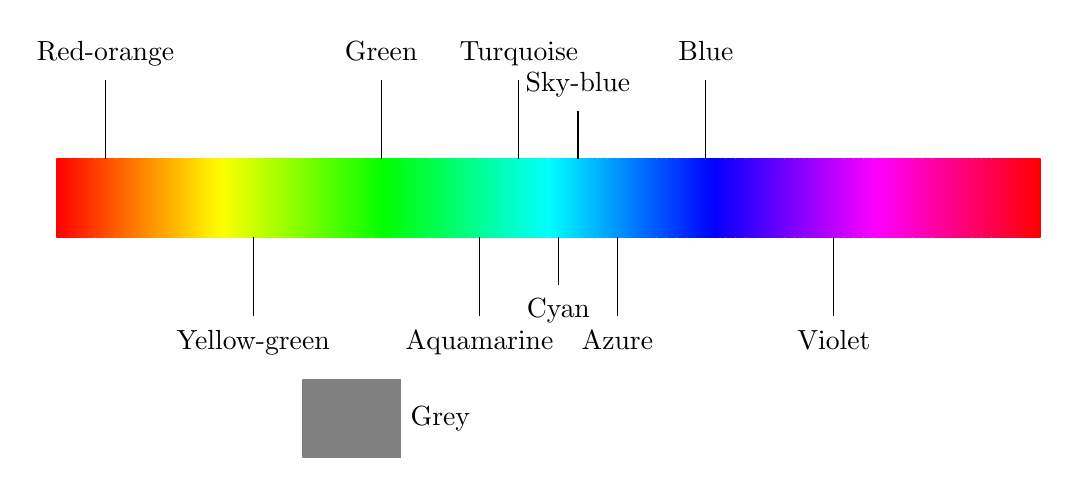
\begin{tikzpicture}[x=1.25mm,y=1mm]
    \definecolor{leftcolour}{hsb}{0,1,1}
    \definecolor{rightcolour}{hsb}{1,1,1}
    \foreach \pos in {0,...,99} {
        \colorlet{current}[rgb]{rightcolour!\pos!leftcolour}
        \pgfmathparse{\pos+1}
        \colorlet{next}[rgb]{rightcolour!\pgfmathresult!leftcolour}
        \shade[
               left color=current,
               right color=next]
           (\pos,0) rectangle +(1,10mm);
    }
    \newcommand{\clabela}[3]{
        \draw (#1, 10mm) -- +(0, #3);
        \pgfmathparse{10 + #3}
        \node[anchor=south, font=\strut] (temp) at (#1, \pgfmathresult) {
            #2
        };
    }
    \newcommand{\clabelb}[3]{
        \draw (#1, 0mm) -- +(0, -#3);
        \node[anchor=north, font=\strut] (temp) at (#1, -#3) {
            #2
        };
    }
    \clabela{5}{Red-orange}{10}
    \clabelb{20}{Yellow-green}{10}
    \clabela{33}{Green}{10}
    \clabelb{43}{Aquamarine}{10}
    \clabela{47}{Turquoise}{10}
    \clabelb{51}{Cyan}{6}
    \clabela{53}{Sky-blue}{6}
    \clabelb{57}{Azure}{10}
    \clabela{66}{Blue}{10}
    \clabelb{79}{Violet}{10}
    \shade[left color=Gray, right color=Gray]
        (25, -18) rectangle (35, -28);
    \node[anchor=west, font=\strut] (grey) at (35, -23) {
        Grey
    };
\end{tikzpicture}

Note that ``grey'' refers generically to a loss of chroma. There is no distinction between a decrease in saturation and a decrease in value.

\lname{} works with colour \emph{transitions}, not static colours. See table \ref{tab:colourtrans}.

\begin{table}[ht]
    \caption{Colour transitions in \lname. Each row represents a different starting colour; each column represents a different ending colour. \label{tab:colourtrans}}
    \centering
    \begin{tabular}{
            l|
            >{\kardinal}l>{\kardinal}l>{\kardinal}l
            >{\kardinal}l>{\kardinal}l>{\kardinal}l
            >{\kardinal}l>{\kardinal}l>{\kardinal}l
            >{\kardinal}l>{\kardinal}l}
        & \textnormal{RO} & \textnormal{YG} & \textnormal{Gn} &
        \textnormal{Aq} & \textnormal{Tu} & \textnormal{Cy} &
        \textnormal{SB} & \textnormal{Az} & \textnormal{Bl} &
        \textnormal{Vi} & \textnormal{Gy} \\
        \hline
        RO & has & mek & d\^yen & fal & s\^hir & pul & be\^ot & mal & f\^xo\^ep & ten\^g & mi \\
        YG & wik & ru\^om & xop & di\^ul & n\^gi\^os & tek & n\^yar & f\^het & tse\^on\^y & yep & pu\^o \\
        Gn & .u\^ik & t\^yul & jek & cum & go\^et & nu\^il & bon\^y & xe\^ot\^y & si\^ul & s\^hu\^os & ko \\
    \end{tabular}
\end{table}

These are abstract nouns.

\appendix

\chapter{Listings of programs}

\section{workfiles/7/tides.sage}
\label{sec:listingtides}

\texttt{
    \lstinputlisting[language=Python]{workfiles/7/tides.sage}
}

\section{workfiles/7/bins.pl6}
\label{sec:listingbins}

\texttt{
    \lstinputlisting[language=Perl]{workfiles/7/bins.pl6}
}

\section{workfiles/7/conno.pl6}
\label{sec:listingconv}

\texttt{
    \lstinputlisting[language=Perl]{workfiles/7/conno.pl6}
}

\section{workfiles/7/count-days.pl6}
\label{sec:listingdays}

\texttt{
    \lstinputlisting[language=Perl]{workfiles/7/count-days.pl6}
}

\chapter{Arithmetic in base $v$}

This chapter describes algorithms for performing arithmetic operations in Lek-Tsaro's number system.

\section{Operations on small numbers}

\subsection{Additions}

If both addends are smaller than 4199, then it is sufficient to use mixed-base addition:

\begin{tabular}
    {>{\kardinal}r>{\kardinal}r>{\kardinal}r>{\kardinal}r}
    & & \small{1} & \\
    & 4 & T & 9 \\
    & 7 & 3 & N \\
    \hline
    & T & N & 6 \\
\end{tabular}

\begin{tabular}
    {>{\kardinal}r>{\kardinal}r>{\kardinal}r>{\kardinal}r}
    \small{1} & \small{1} & & \\
    & 2 & 6 & 5 \\
    & X & F & 3 \\
    \hline
    1 & 2 & 4 & 8
\end{tabular}

\subsection{Subtraction}

If both of the operands are smaller than 4199, then it is sufficient to use mixed-base subtraction.

\begin{tabular}
    {>{\kardinal}r>{\kardinal}r>{\kardinal}r>{\kardinal}r}
    & \small{6} & \small{13.} & \\
    & \cancel{7} & \cancel{3} & N \\
    & 4 & T & 9 \\
    \hline
    & 2 & X & 5
\end{tabular}

\subsection{Determining parity}

A number less than 4199 is even iff the sum of its digits in base $v$ is even -- that is, either none of its digits are odd, or if exactly two are.

\subsection{Dividing by two}

If a number's base-$v$ representation contains only even digits, then divide each digit by two.

If the representation has two odd digits, then take advantage of the identities

\begin{align*}
    11_v / 2 &= 9_v \\
    101_v / 2 &= 99_v \\
    110_v / 2 &= T0_v
\end{align*}

This operation is written as \hortho{m}, short for \hortho{myane} ``one half''. Thus, in hacm:

\begin{itemize}
    \item \textkardinal{m11 = 9}
    \item \textkardinal{m101 = 99}
    \item \textkardinal{m110 = T0}
\end{itemize}

\subsection{Multiplication}

With the previous two operations, it is now possible to use peasant multiplication to multiply small numbers.

\section{Operations on larger numbers}

\subsection{Addition}

For some $i \in \mathbb{N}$, and two numbers number $a = x_a :^i y_a$ and $b = x_b :^i y_b$, we take advantage of the fact that

\begin{align}
    x_a :^i y_a + x_b :^i y_b &=
        (x_a + 1) :^i y_a + (x_b - 1) :^i y_b + (x_a - x_b + 1) \\
    x_a :^i y_a + x_b :^i y_b &=
        (x_a + x_b) :^i y_a + 0 :^i y_b + x_a \cdot x_b \\
    &= (x_a + x_b) :^i (y_a + y_b) + x_a \cdot x_b
\end{align}

%compute the two intermediate sums $\chi = x_a + x_b = x_\chi :^i y_\chi$ and $\psi = y_a + y_b = x_\psi :^i y_\psi$.

\chapter*{Romanisation}

In this text, the romanisation is used only to transcribe names into English. Whenever possible, the hacmisation should be used.

\begin{table}[h]
    \caption{The consonants of \lname. \label{table:hconsr}}
    \centering
    \begin{tabular}{|l|l|l|l|l|l|}
        \hline
        & \textnormal{Bilabial} & \textnormal{Alveolar} & \textnormal{Palatal} & \textnormal{Velar} & \textnormal{Glottal} \\
        \hline
        Nasal & m & n & ñ & ŋ & \invalid \\
        Plosive & p b & t d & ť ď & k g & ' \\
        Fricative & f & s & š & h & \\
        (coarticulated) & þh & fh & & fš & \invalid \\
        Affricate & & ts & tš & & \\
        Lateral fricative & \invalid & ł & & & \invalid \\
        Approximant & & r & j & w & \\
        Lateral approximant & \invalid & l & & & \invalid \\
        Trill & & ř & & \invalid & \invalid \\
        \hline
    \end{tabular}
\end{table}
\begin{table}[h]
\centering
    \caption{The vowels of \lname. \label{table:hvowsr}}
    \begin{tabular}{|l|l|l|}
        \hline
        \textnormal{Spread} & \textnormal{Half-rounded} & \textnormal{Rounded} \\
        \hline
        i & y & ŷ \\
        ï & u & û \\
        e & & ö \\
        ë & & o \\
        a & & \\
        \hline
    \end{tabular}
\end{table}

Rod signs are represented by the Arabic digits \ortho{1 2 3 4 5 6 7 8} attached to the end of the verbs they encompass. Proper words are preceded by a backslash \ortho{\bs{}}.

\ortho{ŋ} should be capitalised as \ortho{Ŋ} only if one can depend on the majuscule glyph appearing like an N with a hook. Otherwise, it should be spelled \ortho{Ng}.

\chapter{Dictionary}

\begin{multicols}{2}
    \input{7/dict/dict.tex}
\end{multicols}

\end{document}
